%% Los cap'itulos inician con \chapter{T'itulo}, estos aparecen numerados y
%% se incluyen en el 'indice general.
%%
%% Recuerda que aqu'i ya puedes escribir acentos como: 'a, 'e, 'i, etc.
%% La letra n con tilde es: 'n.

\chapter{Requirements}
\newpage

In this chapter, it will be explained the requirements acquired after analysing the needs of the users. It is important to say that this analysis is made before designing the main system.\\

Before designing the main system, it was needed to have some interviews with the users that were going to use the system. We listened to all their desires to obtain a good solution.\\

The solution was obtained after doing a good analysis of the tools available for developing Informatic Systems. This solution is not the only one, it is possible to get other solutions, but in this project, we decided to developed the purposed solution because it was affordable.

\section{User requirements}

This section explains the process followed to obtain information about the needs of the user. Here it is explained how the process was made and the steps that we followed to get the information to develop the purpose system.\\

To do this process, it was needed to organize meetings with one of the potential users of the system. It was necessary to organize several meetings to obtain all the requirements of the system. But before organizing all the interviews, it was needed to decide the questions that we had to ask to the users. These questions are described in the following points.

\begin{itemize}

\item \textit{What does the user need?} This is one of the most important things we need to ask to the user. We need to know exactly the desires of the user to check the requirements and, after that, decide if the project is affordable or not.

\item \textit{Who is going to use the system?} This question is needed when we want to know the profiles of the users that are going to use the system. It is important to know if the user has experience with systems similar to the chosen solution. With this information we have an idea about the knowledge of the users and how must be the system for the different users that are going to use it.

\item \textit{When does the user want to get the results?} This question is used when there is a limited requirement related to time. In this case, there is a limit of time established by the user. The user needs to obtain the information as soon as possible.

\item \textit{How does the user want the results?} The user explains how must be the results. It is important this question, because apart of having the results, the user needs to manage the information obtained. Also, it is important the chosen format of the information.

\item \textit{Where does the user want to have access to the system?} With this question we delimit if the system has to be accessible from everywhere or not.

\item \textit{Why does the user need the system?} This is one of the most important questions. It is important to know why the user wants the system, because it is important to analyze all the available tools.

\end{itemize}

After obtaining the answers to all these questions, we have an idea about how must be the system that the users want. The user wants a customized and simple system to query information about materials and to get fast results to do analysis.\\

It is considered an affordable project because it is possible to solve this problem with the available technology.

\subsection{Measure requirements}

It is important to know how must be the requirements linked to measures. The user gave us some information about the possible sensors that could be used to develop the required system.\\

The user does not need complex sensors because the user only wants to estimate information and compare the results with other technologies available in the market.\\

It is important to say that the information obtained by the sensors must be accessible for all the users. This information has to be interpreted with known values to use it for other studies.

\subsection{Access requirements}

The system has to be accessible for the users that are going to access to the system. It is important to explain how to access to the system and the limitations presented by the system.\\

Mobility and comfort are other requirements to consider. We decided to develop a system accessible from different devices like computers, mobile phones or tables.\\

To satisfy this requirement we established that a wireless network would be enough to have access to all the information obtained by the system.

\subsection{Functionality requirements}

The system has to monitor the information registered from sensors every-time. The system has to be available every time.\\

It is important to register information about the studied materials. The objective of monitoring during long period of times is to get better results in the studies.\\

The control of the system is important because it is possible to detect if the system crashes. Also, it is possible to know the reasons of the problems presented to solve them easily.

\section{Technical requirements}

This section is dedicated to describe the requirements related with the physical system and the technology used to develop the purpose system.\\

Here there is an explanation about why it was decided to use the technology described and the features of the designed system. This information makes easier to decide which technology is appropriated to design the system.\\

The designer has to think if the chosen technology satisfies the needs of the users.

\subsection{Hardware requirements}

This section is dedicated to explain the requirements of the hardware used by the system.\\

The hardware has to be simple to use and transparent for the users. The users do not mind the election of the designer, they just want to use the system and do their work as better as possible.\\

The hardware has to be configurable because the user has a customized configuration to work. It should respond to the needs of the users.\\

The selected hardware has to have an easy deployment. It should be deployed everywhere, although the conditions are not the best for a normal system. The system has to work normal although there are in the ambient dust, noise or different item that can make interferences in the system.

\subsection{System requirements}

The system has to be accessible for the users. The user can query information without having a knowledge about how the systems works internally. The user does not need to configure anything in the system.\\

The system has to be auto-configured when the user wants to use it. It implies that it should be automatized and prepare to work every-time and every-where.\\

An important feature of the system is easy way to upgrade and its management. The system should be prepared for improvements if the user needs to upgrade it.

\subsection{Software requirements}

The software has to work transparently to the user. The user must not know how it works internally.\\

The software obtains information about some sensors. It stores the information into a system that is able to manage information. This information is accessible to the user. Also, the information is interpreted according to the requirements of the user.\\

It should be improvable and upgradeable if the needs of the users change.

\section{Planning used in this project}

One of the most important things needed to consider in a project is the existence of a Project Management. In this project, it was necessary to plan different scheduled meetings (to know the needs of the client), calculate timings related to investigation and analysis of the different alternatives which are interesting to apply to this project. Also, considering different death lines it is an important requirement (implementation plan).\\

It was important to consider the time needed to maintain the system after finishing its deployment and how to prepare the client to use the deployed system. Although the client has his/her knowledge to use the system, it was necessary to invest  efforts to prepare a good documentation to allow to future developers to improve and to manage the full system.\\

If we have to enumerate the different things we needed to consider, the most important points are the following.

\begin{itemize}
\item Time needed to know the needs of the client.
\item Time inverted to invest the correct technology to develop the system.
\item Time inverted to get all the components needed to develop the system.
\item Time inverted to develop a correct implementation plan.
\item Plan different meetings to expose the status of the project.
\item Time needed to develop the solution chose by the stakeholder and the engineer.
\item Resources used to deploy the system.
\item Study the results obtained by the developed system.
\item Time inverted to form the client to use the system.
\item Time inverted to provide a good documentation to the client.
\item Time inverted in tasks related to the maintain of the working system.
\end{itemize}

\subsection{Software development methodology used in this project}

Before starting to do all the tasks needed to develop the \textit{Measure System}, it was necessary to decide which methodology was the appropriate for this project. There are several methodologies we can apply to start the development of this project. The different methodologies we could apply to this project are the following:

\begin{enumerate}

\item Waterfall development. It was discarded since the beginning because there is a low feedback from part of the client. This methodology was not the correct one for this project because the most important thing we consider is that the client has to know what is done in the project and the client has to participate in the development plan.

\begin{figure}[H]
\begin{centering}
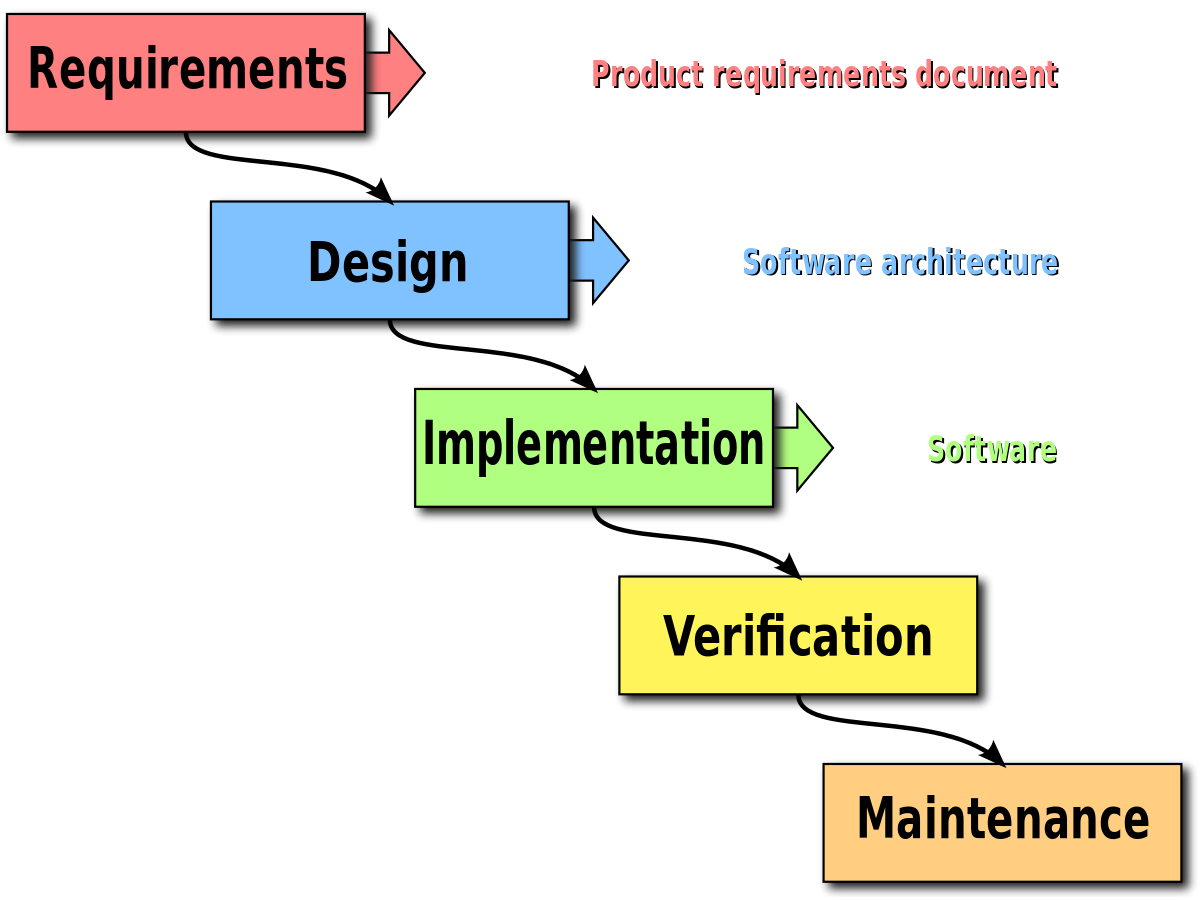
\includegraphics[scale=0.2]{IMGS/waterfall_methodology.png}
\caption{Waterfall methodology \label{Waterfall methodology}}
\end{centering}
\end{figure} 

\item Spiral development. It is an interesting methodology because all the phases of the project are reviewed in all the steps, improving the quality of the final product. The worst thing of this methodology is that the client sometimes cannot participate in the development plan.

\begin{figure}[H]
\begin{centering}
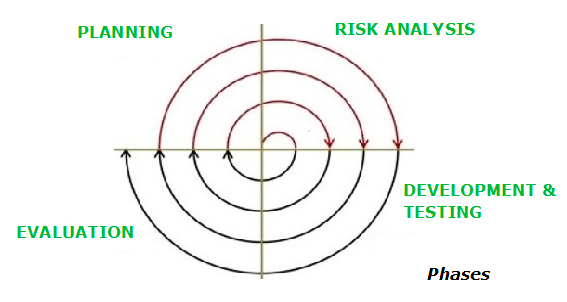
\includegraphics[scale=0.5]{IMGS/spiral-model.jpg}
\caption{Spiral model \label{Spiral model}}
\end{centering}
\end{figure} 

\item V-Model. It is similar to the Spiral development but it has the inconvenient in the cost associated when it is needed to change features at the beginning of the project. Things are changed when the project or the step is in the final state and it has a high cost when it is needed to apply modifications.

\begin{figure}[H]
\begin{centering}
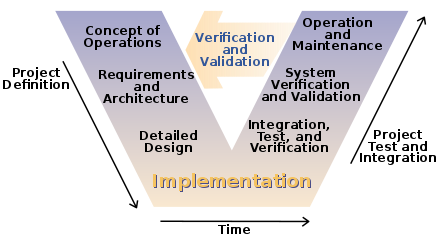
\includegraphics[scale=0.5]{IMGS/v_model.png}
\caption{V model \label{V model}}
\end{centering}
\end{figure} 

\item Scrum. This is one of the fittest methodologies we can apply to this project. The best characteristic of this methodology is that the client can participate in the development process of the product. It is flexible and the costs associated to changes are not high.

\begin{figure}[H]
\begin{centering}
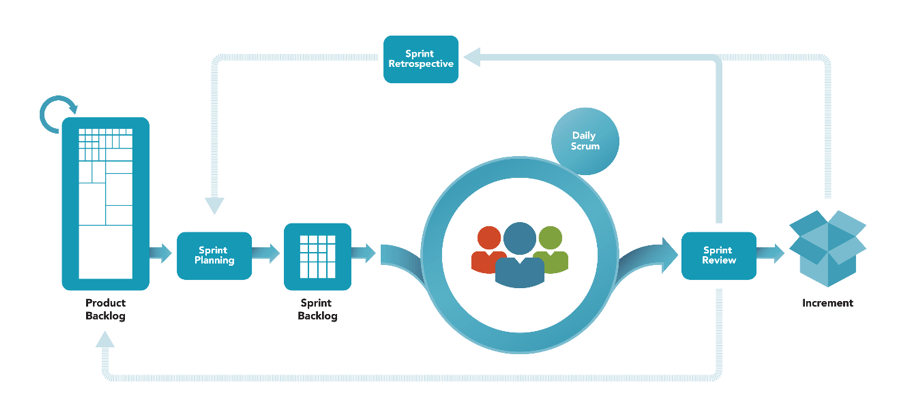
\includegraphics[scale=0.5]{IMGS/Scrum.png}
\caption{Scrum methodology \label{Scrum methodology}}
\end{centering}
\end{figure} 

\end{enumerate}

After knowing the different methodologies we could apply to this project, it was decided to use a hybrid between Spiral development and Scrum model. The main reason to combine both technologies is the possibility to review the project in every step and the importance of the participation of the client in the project. The most important thing is to consider the opinion of the client in every steps because the client is the person which can allow us to develop the correct solution to his/her needs.\\

The other methodologies are not the correct ones to apply to this project because it is more difficult to allow the client to participate in the different phases of the project.

\newpage